% Extended abstract submitted to
% Medical Imaging meets NIPS (workshop)
% https://nips.cc/Conferences/2018/Schedule?showEvent=10928
% https://sites.google.com/view/med-nips-2018/submissions

\documentclass{article}

% if you need to pass options to natbib, use, e.g.:
% \PassOptionsToPackage{numbers, compress}{natbib}
% before loading nips_2018

% ready for submission
\usepackage{nips_2018}

% to compile a preprint version, e.g., for submission to arXiv, add
% add the [preprint] option:
% \usepackage[preprint]{nips_2018}

% to compile a camera-ready version, add the [final] option, e.g.:
% \usepackage[final]{nips_2018}

% to avoid loading the natbib package, add option nonatbib:
% \usepackage[nonatbib]{nips_2018}

\usepackage[utf8]{inputenc} % allow utf-8 input
\usepackage[T1]{fontenc}    % use 8-bit T1 fonts
\usepackage{hyperref}       % hyperlinks
\usepackage{url}            % simple URL typesetting
\usepackage{booktabs}       % professional-quality tables
\usepackage{amsfonts}       % blackboard math symbols
\usepackage{nicefrac}       % compact symbols for 1/2, etc.
\usepackage{microtype}      % microtypography

%%
% Packages inserted by Teo (from Fred's IEEE template):
\usepackage{subfig}
\usepackage{graphicx}


\title{Skin lesion segmentation using a U-Net with\\
  slanted triangular learning rate schedule}

% The \author macro works with any number of authors. There are two
% commands used to separate the names and addresses of multiple
% authors: \And and \AND.
%
% Using \And between authors leaves it to LaTeX to determine where to
% break the lines. Using \AND forces a line break at that point. So,
% if LaTeX puts 3 of 4 authors names on the first line, and the last
% on the second line, try using \AND instead of \And before the third
% author name.

\author{
  Frederico Guth ~ and ~ Teofilo E. deCampos\thanks{http://cic.unb.br/\~{}teodecampos}\\
  Departamento de Ciência da Computação,\\
  Universidade de Brasília (UnB), Bras\'{\i}lia-DF, Brazil, CEP 70910-900 \\
  \texttt{fredguth@fredguth.com}, \texttt{t.decampos@oxfordalumni.org}
  %% examples of more authors
  %% \And
  %% Coauthor \\
  %% Affiliation \\
  %% Address \\
  %% \texttt{email} \\
  %% \AND
  %% Coauthor \\
  %% Affiliation \\
  %% Address \\
  %% \texttt{email} \\
  %% \And
  %% Coauthor \\
  %% Affiliation \\
  %% Address \\
  %% \texttt{email} \\
  %% \And
  %% Coauthor \\
  %% Affiliation \\
  %% Address \\
  %% \texttt{email} \\
}

\begin{document}
% \nipsfinalcopy is no longer used

\maketitle

\begin{abstract}
  In this paper we approach the problem of skin lesion segmentation using a
  convolutional neural network based on the U-Net architecture.
  This network was pretrained with the ImageNet dataset
  and we applied several data augmentation strategies.
  Our experiments show that the use of a slanted triangular learning rate policy
  had a significant impact in its performance.
  We evaluated this method on the ISIC Challenge 2018 - Skin Lesion
  Analysis Towards Melanoma Detection, obtaining threshold Jaccard index of 77.5\%.
\end{abstract}

\section{Introduction}

According to the World Health Organization, between 2 and 3 million
non-melanoma skin cancers and 132,000 melanoma skin cancers occur
globally each year \cite{who}. Despite representing less than 6.5\% of
all skin cancers, melanomas are the most dangerous type, accounting
for aproximately 75\% of all skin cancer related deaths
\cite{who,nature}.

Early detection is critical to increase survival expectancy and visual
inspection still is the most common diagnostic technique.

Deep convolutional neural networks (CNNs) already exceed human
performance in visual classification~\cite{fei}.
In some areas of oncology, such as histological image analysis, CNNs
have also proven to match the performance of experts,
e.g.\ \cite{veta_etal_mia2015}.  In an attempt to improve the
scalability of diagnostic expertise, CNNs have been developed to
locate and classify skin cancers in images with dermatologist-level
accuracy \cite{nature}.

Dermoscopy is a technique for examination of skin lesions that, with
proper training, increase dianostic accuracy from 60\% (unaided expert
visual inspection) to 75\%-84\%~\cite{isic}. The International Skin
Imaging Collaboration (ISIC) has a large-scale publicly acessible
dataset of more than 20,000 dermoscopy images and host an annual
benchmark challenge on dermoscopic image analysis since 2016.  The
challenge comprises 3 tasks of lesion analysis: Segmentation,
Dermoscopic feature extraction and Classification.  In this paper, we
present results on Segmentation, identifying the lesion region in 
dermoscopic images.

\section{The model: U-Net34}
In this paper, we employed U-Net34, which combines insights from both
U-Net and Resnet.

Introduced in 2015, U-Net is an encoder-decoder architecture designed for biomedical image segmentation~\cite{ronneberger_etal_UNet_miccai2015},
with has later been emploied for other image segmentation problems
as well, such as satelite image analysis~\cite{iglovikov}.
In a U-Net, the output is an image with the same dimension of the input,
but with one channel (in the case of binary segmentation problems).
The encoder path is a typical CNN, where each downsampling step doubles
the number of feature channels.
What makes this architecture unique is the decoder path, where each
upsampling step input is a concatenation of the output of the previous
step with the output of the corresponding (same height) downsampling step.
This strategy enables precise localization with a very simple network. 

Resnet is a very successful architecture in several visual classification
tasks~\cite{he}.
It mitigates the degradation problem that happens when very deep
networks starts converging.
Instead of learning a direct mapping $H(x) = y$, it learns the residual
function  $F(x) = H(x)-x$, which can be reframed into
$H(x) = F(x)+x = y$, where $F(x)$ is a stack of non-linear layers and
$x$ is the identity function(input=output).
The formulation of $F(x)+x$ can be implemented by feedforward neural
networks with ``shortcut connections''.
Resnet34, specifically, is composed of an initial convolutional layer,
16 blocks of 2 layers and a final fully connected layer.

Unet34 is the idea of using a pretrained Resnet34 model as a
U-Net encoder path \cite{fastai}. First, every step from the adaptive
pooling onwards is removed, keeping only Resnet backbone.
Then we save the output of results of the initial layer, $3^{rd}$, $8^{th}$,
and $14^{th}$ blocks (of 16 in total). During the upsampling we concatenate the output of those with the ouputs of upsampling steps. We used Adam optimizer and Binary Cross Entropy with Logits as the loss function.

\section{Data and Augmentation}
We used ``ISIC 2018: Skin Lesion Analysis Towards Melanoma Detection'' grand challenge datasets \cite{codella, ham} and no aditional external data. The Segmentation dataset comprises 2597 training images and 101 validation images acquired with a variety of dematoscope types, from different anatomic sites, from sample of patients of different institutions. There are more benign lesions than malignant, but an over-representation of malignacies. Mask images are enconded as grayscale 8-bit PNGs, where ich pixel is either 0, background, or 255, lesion. 

All images were first resized to $128\times128$ pixels, $256\times256$ and $512\times512$; and preprocessed to adjust color balance. Random transformations on input images to agument the dataset were made: dihedral transformation, rotation (up to 44 degrees), zooming (up to 1.05), fliping and random lightining changes. The official training dataset was then splited in 3-folds of training and validation datasets.  



\section{Segmentation Experiments and Training}
\label{sec:seg_training}

CITE THIS: \cite{howard_ruder_acl2018}

Our training strategy was to first train the model with 128x128 images and transfer this learning to train the same model with images with 256 x 256 images. We would suggest using the same strategy to go from 256x256 to 512 x 512 images, but due to GPU memory constraints, we did not manage to acccomplish this last step.

\begin{figure}
  \centering
  \subfloat[Learning Rate vs Validation Loss (Learning Rate Optimization)]{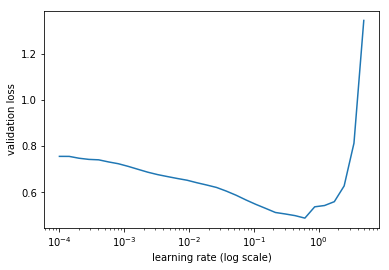
\includegraphics[width=.5\columnwidth]{LR_find.png}\label{lrfind}}
  \subfloat[Iterations vs Learning Rate (cyclical learning rate policy)]{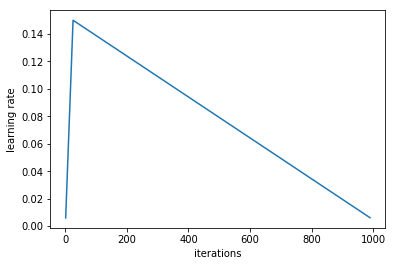
\includegraphics[width=.5\columnwidth]{lr_cycle.png}\label{sconv}}\hfil
  \subfloat[Epoch vs Accuracy (superconvergence)]{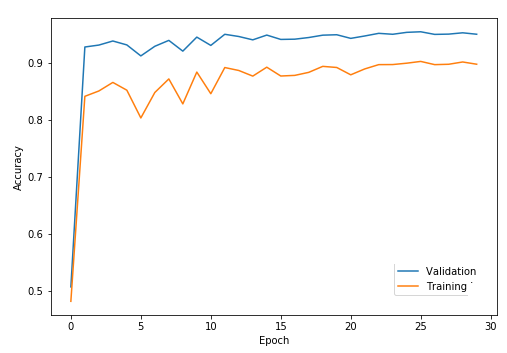
\includegraphics[width=0.6\columnwidth]{accuracy_epoch.png}}
\caption{Learning rate optimization strategy}\label{lr_find_chart}
\end{figure}

The training procedure was the same on 128x128 and 256x256:
\begin{enumerate}
  \item Freeze the first layer group.
  \item \label{lr_find}Define the optimal learning rate with the method proposed by \cite{leslie} and implemented by \cite{fastai}, where one batch is trained with different learning rates, starting at very low and linearly increasing it at every iteration and ploting a chart of the learning rate versus loss (see figure \ref{lrfind}).
  \item \label{superconvergence}We use the 1 cyclical learning rate policy (figure \ref{sconv}), also proposed by \cite{leslie}, to obtain training convergence in only 30 epochs (superconvergence).
  \item Unfreeze the model, keeping only the batch normalization layers frozen, and repeat steps \ref{lr_find} and \ref{superconvergence}.
\end{enumerate}

It would be advisable to use a loss function more similar to the avaliation criteria. As jaccard is not differentiable, one could use a soft jaccard variation\cite{iglovikov}. However, in our priliminar trials the implemented soft jaccard did not improve over the Binary Cross Entropy with Logits loss function and we decided to keep the later. 

We developed two strategies for Task 1:
\emph{BestDice}: This strategy just predicts the input with the model that presented the best dice index on the validation of our splited training dataset. 
\emph{Ensemble}: We used the 3-folds of our training dataset and trained with BestDice model and ensemble than to give a prediction. 

\subsection{Segmentation Results}

\begin{figure}
\centering
\subfloat[Good Result Sample\label{good}]{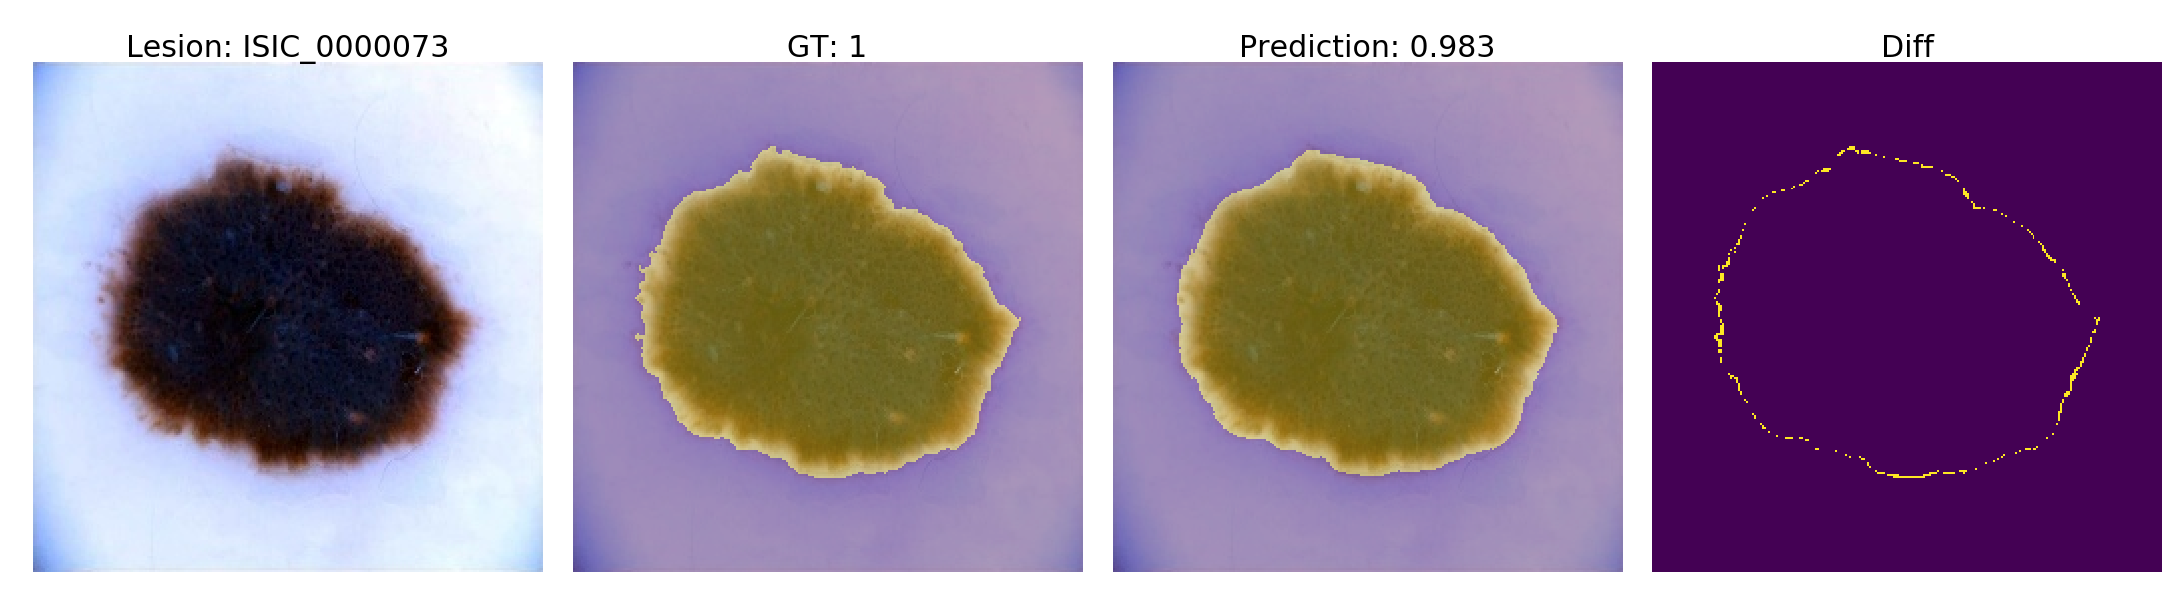
\includegraphics[width=\columnwidth]{good_result.png}}\hfil
\subfloat[Bad Result Samples]{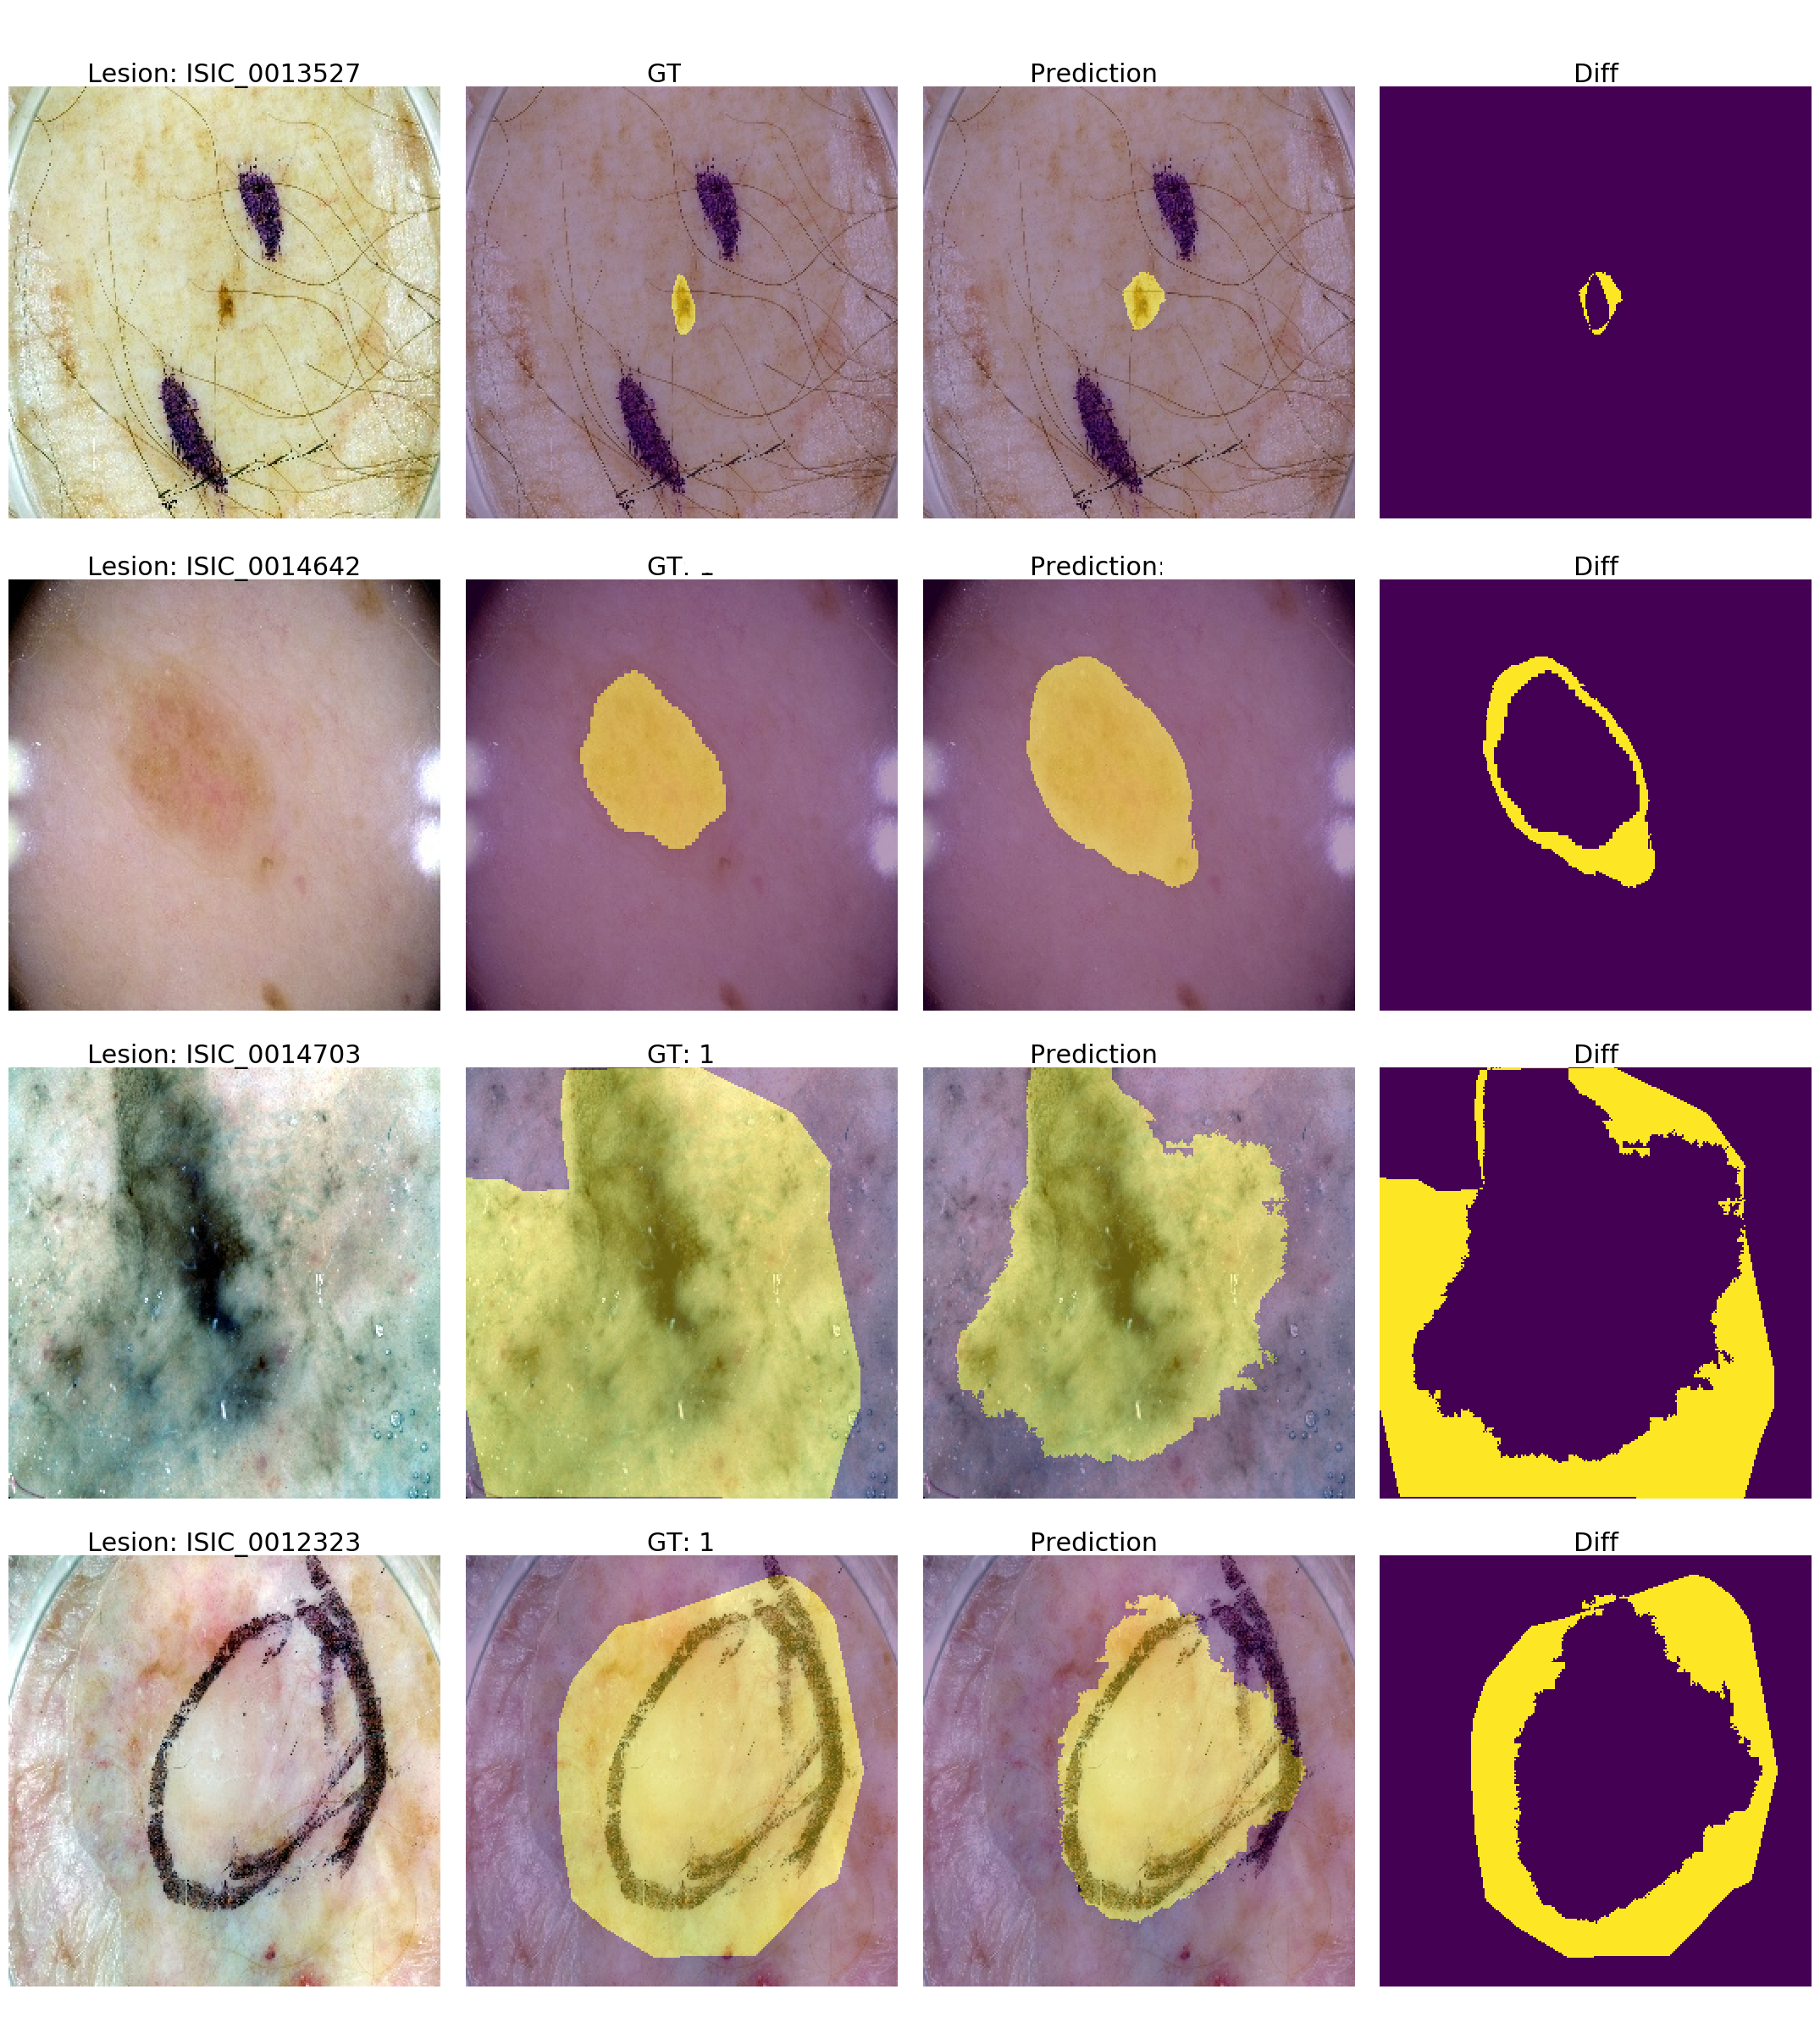
\includegraphics[width=\columnwidth]{bad_results.png}}
\caption{Qualitative assessment of segmentation result}\label{result_samples}
\end{figure}

The best result on our validation set was obtained using the Ensemble strategy.  It achieves a 85.39\% Jaccard index and 78.43\% Threshold Jaccard index (with cut at 65\%). Surprisingly, it did not score so well with the online score and given official validation set, scoring 71.4\%.  The small size of the official validation set and the threshold at 65\% may be the reason for that (one change in prediction from 64\% or 66\% Jaccard makes a huge difference in the average threshold jaccard index). The BestDice strategy achieved an online score of 75.5\% with the official validation set.   Anyway, the top ranked participant in 2017 achieved an average Jaccard Index of 76.5\%, which should be compared with our 85.39\% score.

Visually the best segmentations are almost indentical to the ground truth (see Figure \ref{good}). But we can learn even more from our mistakes. Analysing the worse segmentations there are cases where as non specialists is hard to say if the algorithm was wrong or the ground truth was; there are cases where our algorithm got confused by the pen marker or the glass used by the doctor; and it is clear that in general it doesn't do a good job when the lesion is small relative to the overall image. 




\medskip

\small
\bibliographystyle{plain}
\bibliography{references}

\end{document}
